% ============================================================
% §4  Results
% ============================================================
\section{Results}
\label{sec:results}

I report three complementary views of the benchmark: the omnibus
statistical ranking, per-problem median regret, and regret trajectories.
Together they tell a consistent story: the 240 BO runs partition the
four strategies into two statistically separated equivalence classes.

% ----------------------------------------------------------
\subsection{Omnibus Statistical Test}
\label{sec:friedman}

The Friedman test strongly rejects the null hypothesis of equal expected
ranks across the four strategies:
$\chi^2(3) = 128.82$, $p = 9.73 \times 10^{-28}$ ($N = 60$ blocks,
$k = 4$).
Average ranks are
UCB $= 1.39$, EI $= 1.76$, Uncertainty $= 3.38$, Random $= 3.48$.

The rank ordering partitions into two well-separated groups.
The gap between EI (1.76) and Uncertainty (3.38) is $1.62$, more than
two and a half times the critical difference $\mathrm{CD} = 0.61$.
Within each group the gaps are small: UCB and EI differ by $0.37$
(below CD), and Uncertainty and Random differ by $0.10$ (far below CD).

% ----------------------------------------------------------
\subsection{Nemenyi Pairwise Comparisons}
\label{sec:nemenyi}

All six pairwise Nemenyi comparisons at $\alpha = 0.05$ are reported in
Table~\ref{tab:nemenyi} and visualized in the Critical Difference diagram
(Figure~\ref{fig:cd}).

\begin{table*}[t]
\centering
\caption{Nemenyi post-hoc $p$-values.
  NS = not significant at $\alpha = 0.05$; ${}^{***}$ = $p < 10^{-6}$.
  Two distinct equivalence classes emerge: \{UCB, EI\} and
  \{Uncertainty, Random\}.}
\label{tab:nemenyi}
\begin{tabular}{lcccc}
\toprule
         & UCB     & EI      & Uncertainty & Random \\
\midrule
UCB      & —       & 0.404 \scriptsize{(NS)} & $<\!10^{-6}$ ${}^{***}$ & $<\!10^{-6}$ ${}^{***}$ \\
EI       &         & —       & $<\!10^{-6}$ ${}^{***}$ & $<\!10^{-6}$ ${}^{***}$ \\
Uncertainty &      &         & —           & 0.974 \scriptsize{(NS)} \\
Random   &         &         &             & — \\
\bottomrule
\end{tabular}
\end{table*}

The results define two equivalence classes:
\begin{itemize}[nosep]
  \item \textbf{Balanced strategies}: \{UCB, EI\} — statistically
    indistinguishable from each other ($p = 0.404$), both significantly
    better than the pure-exploration strategies ($p < 10^{-6}$).
  \item \textbf{Pure-exploration strategies}: \{Uncertainty, Random\} —
    statistically indistinguishable from each other ($p = 0.974$), both
    significantly worse than the balanced strategies ($p < 10^{-6}$).
\end{itemize}

The most striking result is the Uncertainty–Random tie.
Uncertainty selects points by maximizing posterior standard deviation
using the same fitted GP as EI and UCB; it is not a blind strategy.
Yet its rank ($3.38$) is statistically indistinguishable from Random
($3.48$, $p = 0.974$).
This isolates the contribution of exploitation: the GP's uncertainty
estimate, used \emph{without} the posterior mean, provides no
measurable advantage over blind Sobol sampling.

\begin{figure*}[t]
  \centering
  
\includegraphics[width=0.82\linewidth]{figures/exp_03_cd_diagram.png}
  \caption{Critical Difference diagram ($\alpha = 0.05$, $k = 4$,
    $N = 60$, $\mathrm{CD} = 0.61$).
    Horizontal bars connect strategies that are not significantly
    different.  Two separate cliques are visible: \{UCB, EI\}
    (left, lower ranks = better) and \{Uncertainty, Random\}
    (right, higher ranks = worse).}
  \label{fig:cd}
\end{figure*}

% ----------------------------------------------------------
\subsection{Per-Problem Median Regret}
\label{sec:per-problem}

Table~\ref{tab:median} reports median final regret across 10 seeds for
each problem–strategy pair.
I report median rather than mean because several seeds produce
outlier-high regret on certain problem–strategy combinations; for
example, EI on Borehole has a mean final regret of $8.63$ (inflated by
two outlier seeds) but a median of only $2.41$.
Median is more representative of typical performance and robust to
heavy-tailed distributions.

\begin{table*}[t]
\centering
\caption{Median final simple regret after 20 iterations, 10 seeds.
  Bold = best per row.  Ordered by dimension.
  All problems are maximization; lower regret is better.}
\label{tab:median}
\begin{tabular}{lcccc}
\toprule
Problem ($d$) & EI & UCB & Uncertainty & Random \\
\midrule
Branin (2)       & 0.026 & \textbf{0.015} & 2.676 & 0.920 \\
SixHumpCamel (2) & \textbf{0.057} & 0.287 & 0.936 & 0.924 \\
Hartmann-6 (6)   & \textbf{0.183} & 0.254 & 1.913 & 1.802 \\
Piston (7)       & 0.016 & \textbf{0.001} & 0.033 & 0.395 \\
Borehole (8)     & 2.409 & \textbf{0.424} & 5.747 & 111.642 \\
Ackley-10D (10)  & \textbf{3.800} & 4.295 & 8.441 & 8.272 \\
\midrule
Avg.\ rank & 1.76 & \textbf{1.39} & 3.38 & 3.48 \\
\bottomrule
\end{tabular}
\end{table*}

Several patterns are visible across the table.
First, the balanced strategies (EI, UCB) lead on every single problem;
the pure-exploration strategies (Uncertainty, Random) never win a row.
Second, the magnitude of the advantage varies substantially with problem
structure.
On Borehole (8D, engineering), UCB's median regret ($0.42$) is
$263\times$ lower than Random's ($111.6$), reflecting the structured,
near-monotone response surface that a well-calibrated GP can exploit.
On Ackley-10D (synthetic, highly multimodal), EI's median ($3.80$)
is only $2.2\times$ lower than Random's ($8.27$), consistent with
the curse of dimensionality degrading GP calibration at this budget.
Third, among the balanced strategies, neither EI nor UCB consistently
dominates: UCB ranks first on four of six problems, EI on two, and
their average ranks (1.39 vs.\ 1.76) are not significantly different
(Nemenyi $p = 0.404$).

% ----------------------------------------------------------
\subsection{Regret Trajectories}
\label{sec:trajectories}

Figures~\ref{fig:borehole} and~\ref{fig:ackley} show mean regret
trajectories ($\pm$ one standard deviation) across seeds for the two
most contrasting problems.

\begin{figure}[tb]
  \centering
  
\includegraphics[width=\linewidth]{figures/exp_02_borehole_strategies.png}
  \caption{Mean regret $\pm$ std over 20 iterations on Borehole (8D).
    EI and UCB converge rapidly while Uncertainty and Random show
    negligible improvement.
    The large EI std band is driven by two outlier seeds with elevated
    final regret, inflating the mean well above the median ($8.63$
    vs.\ $2.41$).}
  \label{fig:borehole}
\end{figure}

\begin{figure}[tb]
  \centering
  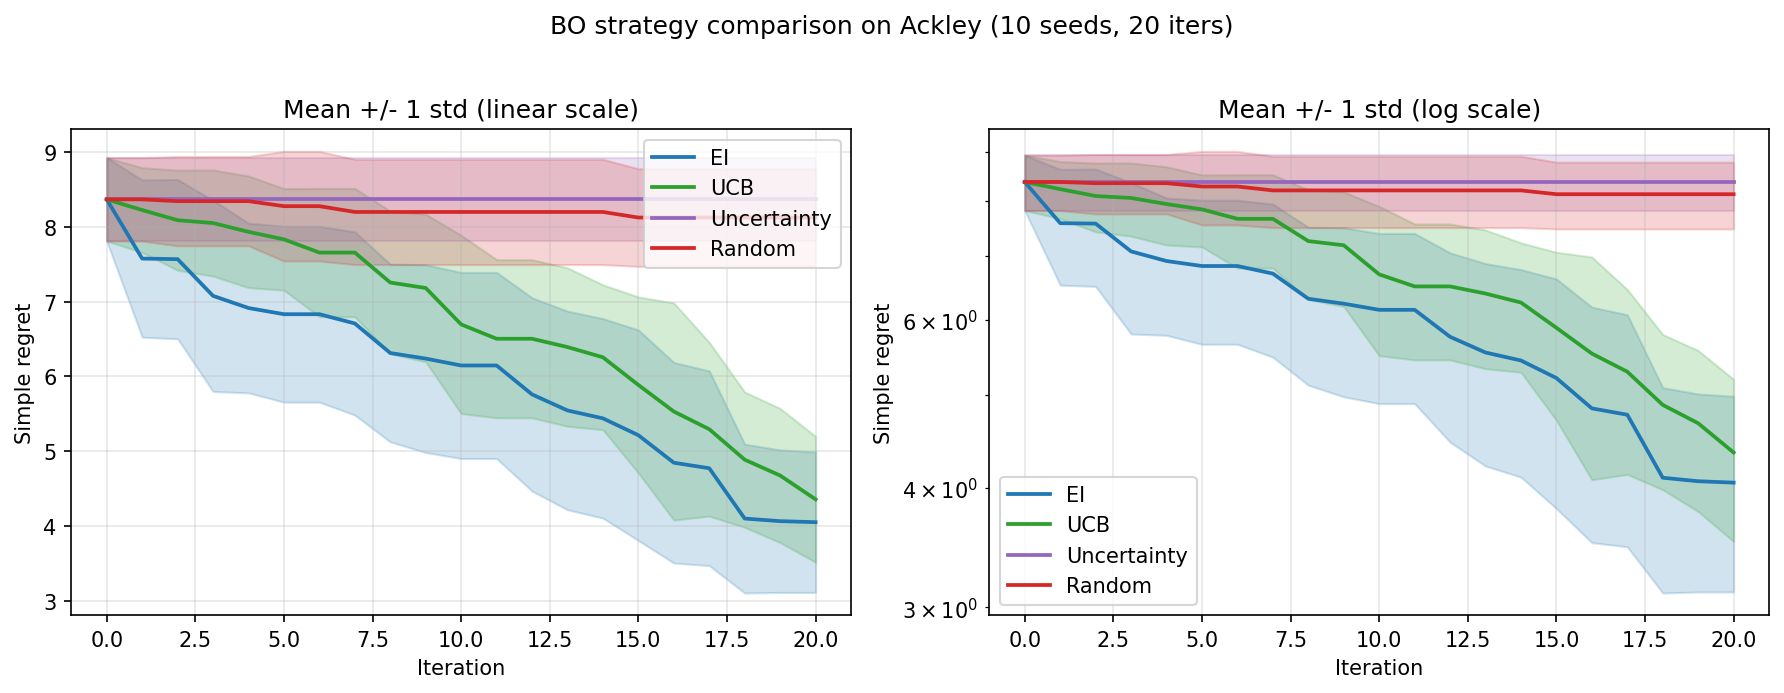
\includegraphics[width=\linewidth]{figures/exp_02_ackley_strategies.png}
  \caption{Mean regret $\pm$ std over 20 iterations on Ackley-10D.
    All four strategies remain at high regret; EI and UCB show a
    marginal but consistent advantage over pure-exploration strategies.
    The narrow gap between balanced and pure-exploration strategies
    illustrates dimensionality-driven degradation of GP calibration.}
  \label{fig:ackley}
\end{figure}

% ----------------------------------------------------------
\subsection{Effect of Dimensionality}
\label{sec:dimension}

To quantify how the EI–Random gap changes with dimensionality I use
mean final regret, which captures tail behavior that median suppresses.
On Branin (2D), EI achieves a mean regret of $0.034$ against Random's
$1.58$, a ${\approx}47{\times}$ advantage.
On Ackley-10D, EI achieves $4.05$ against Random's $8.13$, a
${\approx}2{\times}$ advantage—a more than 20-fold reduction in relative
gain over eight additional dimensions.

This collapse in advantage is consistent with the theoretical analysis
in \citet{shahriari2016taking}: in high dimensions the GP surrogate
requires exponentially more observations to achieve accurate uncertainty
estimates, and the 20-iteration budget used here is far from sufficient
to cover the $[-5, 5]^{10}$ search space.
The Ackley function has no low-effective-dimensionality structure that
could be exploited through embeddings or variable selection, making it a
worst-case scenario for GP-based BO at this budget.
